%%%%%%%%%%%%%%%%%%%%%%%%%%%%%%%%%%%%%%%%%
% Beamer Presentation
% LaTeX Template
% Version 1.0 (10/11/12)
%
% This template has been downloaded from:
% http://www.LaTeXTemplates.com
%
% License:
% CC BY-NC-SA 3.0 (http://creativecommons.org/licenses/by-nc-sa/3.0/)
%
%%%%%%%%%%%%%%%%%%%%%%%%%%%%%%%%%%%%%%%%%

%----------------------------------------------------------------------------------------
%	PACKAGES AND THEMES
%----------------------------------------------------------------------------------------

\documentclass{beamer}

\mode<presentation> {

% The Beamer class comes with a number of default slide themes
% which change the colors and layouts of slides. Below this is a list
% of all the themes, uncomment each in turn to see what they look like.
\usepackage[utf8]{vietnam}	
%\usetheme{default}
%\usetheme{AnnArbor}
%\usetheme{Antibes}
%\usetheme{Bergen}
%\usetheme{Berkeley}
%\usetheme{Berlin}
%\usetheme{Boadilla}
%\usetheme{CambridgeUS}
%\usetheme{Copenhagen}
%\usetheme{Darmstadt}
%\usetheme{Dresden}
%\usetheme{Frankfurt}
%\usetheme{Goettingen}
%\usetheme{Hannover}
%\usetheme{Ilmenau}
%\usetheme{JuanLesPins}
%\usetheme{Luebeck}
\usetheme{Madrid}
%\usetheme{Malmoe}
%\usetheme{Marburg}
%\usetheme{Montpellier}
%\usetheme{PaloAlto}
%\usetheme{Pittsburgh}
%\usetheme{Rochester}
%\usetheme{Singapore}
%\usetheme{Szeged}
%\usetheme{Warsaw}

% As well as themes, the Beamer class has a number of color themes
% for any slide theme. Uncomment each of these in turn to see how it
% changes the colors of your current slide theme.

%\usecolortheme{albatross}
%\usecolortheme{beaver}
%\usecolortheme{beetle}
%\usecolortheme{crane}
%\usecolortheme{dolphin}
%\usecolortheme{dove}
%\usecolortheme{fly}
%\usecolortheme{lily}
%\usecolortheme{orchid}
%\usecolortheme{rose}
%\usecolortheme{seagull}
%\usecolortheme{seahorse}
%\usecolortheme{whale}
%\usecolortheme{wolverine}

%\setbeamertemplate{footline} % To remove the footer line in all slides uncomment this line
%\setbeamertemplate{footline}[page number] % To replace the footer line in all slides with a simple slide count uncomment this line

%\setbeamertemplate{navigation symbols}{} % To remove the navigation symbols from the bottom of all slides uncomment this line
}

\usepackage{graphicx} % Allows including images
\usepackage{booktabs} % Allows the use of \toprule, \midrule and \bottomrule in tables

%----------------------------------------------------------------------------------------
%	TITLE PAGE
%----------------------------------------------------------------------------------------

\title[Học tăng cường]{Học tăng cường} % The short title appears at the bottom of every slide, the full title is only on the title page

\author{Phạm Hữu Nghị, Phạm Thanh Sơn\\ Nguyễn Lê Hoàng, Vũ Hải Trường} % Your name
\institute[UCLA] % Your institution as it will appear on the bottom of every slide, may be shorthand to save space
{
Giáo viên hướng dẫn: TS. Nguyễn Thị Ngọc Anh \\ % Your institution for the title page
\medskip
%\textit{john@smith.com} % Your email address
}
\date{\today} % Date, can be changed to a custom date

\begin{document}

\begin{frame}
\titlepage % Print the title page as the first slide
\end{frame}

\begin{frame}
\frametitle{Nội dung} % Table of contents slide, comment this block out to remove it
\tableofcontents % Throughout your presentation, if you choose to use \section{} and \subsection{} commands, these will automatically be printed on this slide as an overview of your presentation
\end{frame}

%----------------------------------------------------------------------------------------
%	PRESENTATION SLIDES
%----------------------------------------------------------------------------------------

%------------------------------------------------
\section{Giới thiệu} % Sections can be created in order to organize your presentation into discrete blocks, all sections and subsections are automatically printed in the table of contents as an overview of the talk
%------------------------------------------------

\begin{frame}
\frametitle{Giới thiệu}
\begin{itemize}
\item Học tăng cường (reinforcement learning) là một lĩnh vực con của học máy, nghiên cứu cách thức một tác tử (agent) trong một môi trường nên chọn thực hiện các hành động nào để cực đại hóa một khoản thưởng (reward).
\item Môi trường thường được biểu diễn dưới dạng một quá trình quyết định Markov trạng thái hữu hạn (Markov decision process - MDP).
\item Trong học tăng cường không có các cặp dữ liệu vào/kết quả đúng, các hành động gần tối ưu cũng không được đánh giá đúng sai một cách tường minh.
\end{itemize}
\end{frame}

\begin{frame}
\frametitle{Giới thiệu}
\begin{figure}[H]
  \begin{center}
    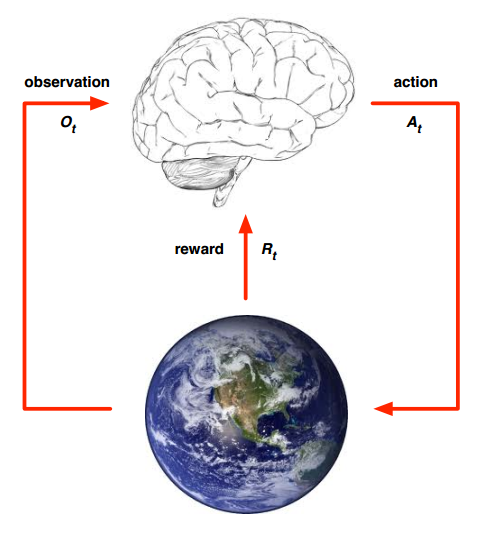
\includegraphics[width=0.6\textwidth]{s1.png}
  \end{center}
  \label{s1}
\end{figure}
\end{frame}

%------------------------------------------------
\section{Quá trình quyết định Markov}
%------------------------------------------------

\subsection{Quá trình quyết định Markov} % A subsection can be created just before a set of slides with a common theme to further break down your presentation into chunks

%------------------------------------------------

\begin{frame}
\frametitle{Quá trình quyết định Markov}
\begin{itemize}
\item Quá trình quyết định Markov với vai trò là môi trường cho học tăng cường.
\item Có tính Markov (tính không nhớ).
\item Hầu hết các bài toán học tăng cường đều có thể biểu diễn thành một quá trình quyết định Markov.
\end{itemize}
\end{frame}

%------------------------------------------------

%\begin{frame}
%\frametitle{Tính Markov}
%\begin{block}{Định nghĩa}
%Trạng thái $S_t$ được gọi là có tính Markov nếu:
%$$\mathbb{P}[S_{t+1}|S_t]=\mathbb{P}[S_{t+1}|S_1,...,S_t]$$
%\end{block}
%\end{frame}

%------------------------------------------------

\begin{frame}
\frametitle{Quá trình quyết định Markov}
Quá trình quyết định Markov gồm 5 thành phần:
$$\mathcal{M}=(\mathcal{S}, \mathcal{A}, \mathcal{P}_.(\cdotp,\cdotp),\mathcal{R}_.(\cdotp,\cdotp),\gamma)$$
Trong đó:
\begin{itemize}
\item $\mathcal{S}$ là một tập các trạng thái.
\item $\mathcal{A}$ là một tập các hành động (ngoài ra, $\mathcal{A}_s$ là tập hữu hạn các hành động có sẵn từ trạng thái $s$).
\item $\mathcal{P}_a(s,s')=Pr(s_{t+1}=s'|s_t=s,a_t=a)$ là xác suất mà hành động $a$ trong thái thái $s$ tại thời gian $t$ sẽ dẫn đến trạng thái $s'$ tại thời gian $t+1$.
\item $\mathcal{R}_a(s,s')$ là phần thưởng trực tiếp (hoặc phần thưởng trực tiếp mong đợi) nhận được sau khi chuyển tiếp sang trạng thái $s'$ từ trạng thái $s$.
\item $\gamma \in [0,1]$ là hệ số chiết khấu, sẽ đại diện cho sự khác biệt quan trọng giữa các phần thưởng tương lai và phần thưởng hiện tại.
\end{itemize}
\end{frame}

\begin{frame}
\frametitle{Bài toán}
\begin{itemize}
\item Bài toán cốt lõi của MDP đó là tìm một "nguyên tắc" cho người ra quyết định: một hàm $\pi$  mà xác định hành động $\displaystyle \pi (s)$ rằng người ra quyết định sẽ chọn khi trong trạng thái s.
\item Mục đích là để chọn ra một nguyên tắc $\pi$ mà sẽ tối đa hóa vài hàm tích lũy của các phần thưởng ngẫu nhiên, điển hình là tổng lợi nhuận:
\end{itemize}
$$\mathcal{R}=\sum_{t=0}^{\infty}{\gamma^{t}R_{a_t}(s_t,s_{t+1})} \qquad (\text{trong đó ta chọn } a_t=\pi (s_t))$$
$\qquad$Trong đó $\gamma$ là hệ số chiết khấu và thỏa mãn $0\leq \gamma \leq 1$.
\end{frame}

\subsection{Hàm giá trị}

\begin{frame}
\frametitle{Hàm giá trị}
\begin{block}{Định nghĩa}
Hàm giá trị $v(s)$ là kỳ vọng lợi nhuận bắt đầu ở trạng thái $s$ và theo nguyên tắc $\pi$
$$v_\pi (s)=\mathbb{E}_\pi [G_t|S_t=s]$$
\end{block}

\begin{block}{Định nghĩa}
Hàm hành động - giá trị $q_\pi (s,a)$ là kỳ vọng lợi nhuận bắt đầu ở trạng thái $s$ thực hiện hành động $a$ và theo nguyên tắc $\pi$
$$q_\pi (s,a)=\mathbb{E}_\pi [G_t|S_t=s,A_t=a]$$
\end{block}
\end{frame}

\begin{frame}
\frametitle{Công thức Bellman}
Hàm giá trị có thể được tách ra thành 2 phần:
\begin{itemize}
\item Phần thưởng $R_{t+1}$
\item Giá trị chiết khấu của trạng thái kế tiếp $\gamma v_\pi (S_{t+1})$
\end{itemize}
\begin{equation}
\begin{split}
v_\pi (s) & = \mathbb{E}_\pi [G_t|S_t = s] \\
& = \mathbb{E}_\pi [R_{t+1} + \gamma R_{t+2} + \gamma^2 R_{t+3} + ... | S_t = s] \\
& = \mathbb{E}_\pi [R_{t+1} + \gamma (R_{t+2} + \gamma R_{t+3} + ...) | S_t = s] \\
& = \mathbb{E}_\pi [R_{t+1} + \gamma G_{t+1} | S_t = s] \\
& = \mathbb{E}_\pi [R_{t+1} + \gamma v(S_{t+1}) | S_t = s] \\
\end{split}
\end{equation}
Tương tự ta có:
$$q_\pi (s,a) = \mathbb{E}_\pi [R_{t+1} + \gamma q_\pi (S_{t+1},A_{t+1}) | S_t = s, A_t =a]$$
\end{frame}

\section{Q-Learning}
\begin{frame}
\begin{block}{Định lý}
Cho quá trình quyết đinh Markov hữu hạn $MDP(\mathcal{X},\mathcal{A},\mathcal{P},r)$
.Hàm mục tiêu:
$$J(x,{A_t})=E\big[ \sum_{t=0}^\infty{\gamma^t R(X_t,A_t)|X_0=x} \big]$$
Thuật toán Q-learning với công thức lặp:
$$Q_{t+1}(s_t,a_t)=Q_t(x_t,a_t)+\alpha_t(x_t,a_t)[r_t +\gamma max_{b \in \mathcal{A}}Q_t(x_{t+1},b)-Q_t(x_t,a_t)]$$
Hội tụ với xác suất bằng 1 tới hàm Q tối ưu:
$$Q^*(x,a)=\sum_{y\in\mathcal{X}}{P(x,a,y)[r(x,a,y)+\gamma V^*(y)]}$$
Trong đó V* là hàm giá trị tối ưu của J:
$$V^*(x)=max_{a\in\mathcal{A}}\sum_{y\in\mathcal{X}}{P(x,a,y)[r(x,a,y)+\gamma V^*(y)]}$$
\end{block}
\end{frame}
\section{Ứng dụng Q-learning}
\begin{frame}
\frametitle{Ứng dụng Q-learning trong game AI }
\begin{figure}[H]
  \begin{center}
    \includegraphics[width=0.7\textwidth]{s3.png}
  \end{center}
  \label{s1}
\end{figure}
\end{frame}


%------------------------------------------------
\section{Kết quả và nhận xét}
%------------------------------------------------


%------------------------------------------------


%------------------------------------------------


%------------------------------------------------


%------------------------------------------------

%------------------------------------------------

\begin{frame}
\Huge{\centerline{The End}}
\end{frame}

%----------------------------------------------------------------------------------------

\end{document}
